\newpage

\subsection{Elenco dei casi d'uso}
%---------------------------- UC1 ---------------------------------

\begin{figure}[H]
    \centering
    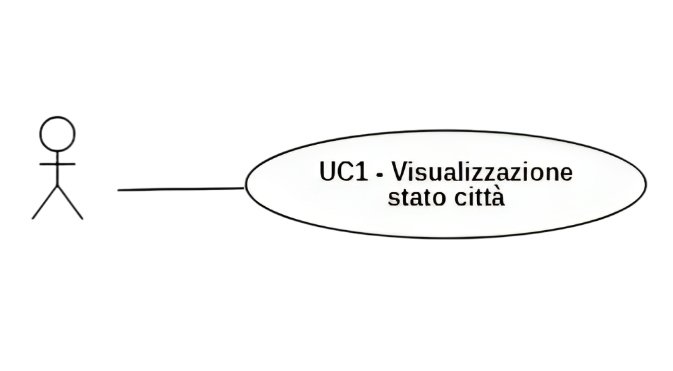
\includegraphics[width=0.9\textwidth]{../Images/uc1.png}
    \caption{UC1 - VISUALIZZAZIONE DASHBOARD}
    \label{fig:UC1}
\end{figure}

\subsubsection{UC1 - VISUALIZZAZIONE DASHBOARD}
\begin{itemize}
    \item \textbf{Attore principale:} Autorità locale.
    \item \textbf{Precondizioni:}
        \begin{itemize}
            \item Il sistema è operativo e accessibile.
        \end{itemize}
    \vspace{0,5cm}
    \item \textbf{Postcondizioni:}
    \begin{itemize}
        \item  L'autorità locale ha una visione aggiornata dello stato di salute della città tramite widget e grafici interattivi aggiornati in tempo reale, una mappa dei sensori presenti nella città e un punteggio di salute relativo alla città.
    \end{itemize}
    \item \textbf{Scenario principale:}
        \begin{enumerate}
            \item L'autorità locale accede alla piattaforma per la visualizzazione della dashboard;
            \item Il sistema elabora le informazioni ricevute dai sensori;
            \item Il sistema imposta la visualizzazione dei widget sulla dashboard.
        \end{enumerate}
    \item \textbf{User story associata:} \\
        Come autorità locale, voglio accedere alla dashboard per visualizzare in tempo reale i dati provenienti dai diversi tipi di sensori presenti nella città. Questo mi consentirà di valutare rapidamente lo stato generale della città e prendere decisioni informate e tempestive sulla gestione delle risorse e sull'implementazione di servizi.
\end{itemize}

%---------------------------- SUB_UC1 ---------------------------------

\begin{figure}[H]
    \centering
    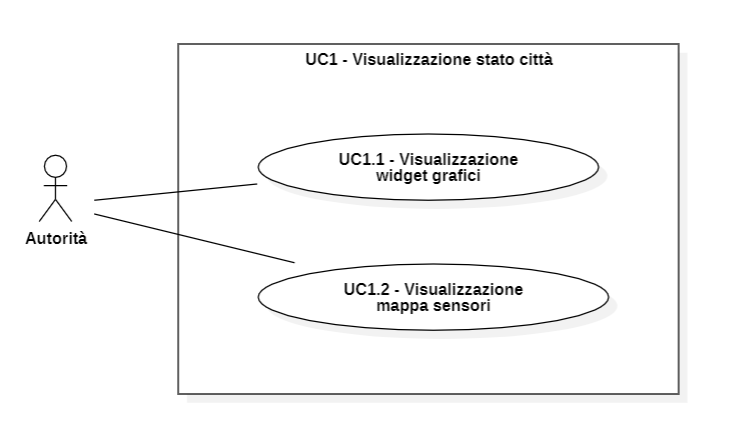
\includegraphics[width=0.9\textwidth]{../Images/uc1_Subcase.PNG} 
    \caption{Sottocasi UC1 - VISUALIZZAZIONE DASHBOARD}
    \label{fig:UC1_sub}
\end{figure}

%---------------------------- UC1.1 ---------------------------------

\subsubsection{UC1.1 - PANORAMICA COMPLESSIVA DEI WIDGET DI MISURAZIONE PER OGNI TIPOLOGIA DI SENSORE}
\begin{itemize}
    \item \textbf{Attore principale:} Autorità locale.
    \item \textbf{Descrizione:} L'autorità locale accede alla dashboard della città e visualizza un widget contente un grafico aggiornato in tempo reale, il quale rappresenta i dati registrati durante la giornata per ogni tipologia di sensore che trasmette al sistema.
    \item \textbf{Scenario principale:}
        \begin{enumerate}
            \item L'utente accede alla piattaforma per la visualizzazione della dashboard della città. (UC1)
            \item Il sistema elabora le informazioni ricevute dai sensori e imposta la visualizzazione di un widget con le misurazioni quotidiane per ogni tipolgia di sensore;
        \end{enumerate}
    \item \textbf{Precondizioni:}
        \begin{itemize}
            \item Nessuna
        \end{itemize}
    \item \textbf{Postcondizioni:}
        \begin{itemize}
            \item L'autorità locale ha una visione di un widget con misurazioni aggiornate in tempo reale, il quale rappresenta i dati registrati durante la giornata per ogni tipologia di sensore.
        \end{itemize}
    \item \textbf{User story associata:}
        \begin{itemize}
            \item Come autorità locale voglio visualizzare widget come le misurazioni aggiornate in tempo reale sui dati registrati durante la giornata per ogni tipologia di sensore nella dashboard.
        \end{itemize}
\end{itemize}


%---------------------------- UC1.2 ---------------------------------

\subsubsection{UC1.2 - Visualizzazione mappa sensori}
\begin{itemize}
    \item \textbf{Attore principale:} Autorità locale.
    \item \textbf{Descrizione:} L'autorità locale accede alla dashboard della città e visualizza una mappa con una visione dei sensori posizionati nella città.
    \item \textbf{Scenario principale:}
          \begin{enumerate}
              \item L'utente visualizza una mappa contenente i sensori nella corretta posizione. (i sensori sono etichettati per riconoscere la tipologia)
          \end{enumerate}
    \item \textbf{Precondizioni:}
          \begin{itemize}
              \item  Almeno un sensore è attivo e ha trasmesso dati;
              \item L'utente si trova nella dashboard della città. (UC1)
          \end{itemize}
    \item \textbf{Postcondizioni:}
          \begin{itemize}
              \item      L'utente ha una visione grafica aggiornata della mappa dei sensori nella città e della loro tipologia.
          \end{itemize}
    \item \textbf{User story associata:}
          \begin{itemize}
              \item Come autorità locale, voglio essere in grado di visualizzare una mappa contenente i sensori attivi e operativi all'interno della città. La mappa deve mostrare chiaramente la posizione di ciascun sensore e devono essere etichettati per consentire un riconoscimento immediato della tipologia di ogni sensore.
          \end{itemize}
\end{itemize}

%---------------------------- UC1.3 ---------------------------------
\newpage

\subsubsection{UC1.3 - VISUALIZZAZIONE WIDGET PUNTEGGIO DI SALUTE}
\begin{itemize}
    \item \textbf{Attore principale:} Autorità locale.
    \item \textbf{Precondizioni:}
        \begin{itemize}
            \item Il sistema è operativo e accessibile.
        \end{itemize}
    \item \textbf{Postcondizioni:}
        \begin{itemize}
            \item L'autorità locale ha una visione aggiornata di un punteggio, un numero intero, rappresentante lo stato di salute della città.
        \end{itemize}
    \item \textbf{Scenario principale:}
          \begin{enumerate}
            \item L'autorità locale accede alla piattaforma per la visualizzazione della dashboard. (UC1)
            \item Il sistema elabora i dati provenienti dai sensori e calcola un punteggio di salute.
        \end{enumerate}
    \item \textbf{User story associata:} \\
        Come autorità locale, desidero visualizzare un punteggio ottenuto tramite una funzione di aggregazione, il quale fornisca una visione immediata di eventuali dati anomali rilevati dai sensori disseminati nella città, al fine di identificare rapidamente situazioni critiche e prendere azioni tempestive per garantire la sicurezza e il benessere della comunità.
\end{itemize}

%---------------------------- SUB_UC1.1 ---------------------------------
\newpage

\begin{figure}[H]
    \centering
    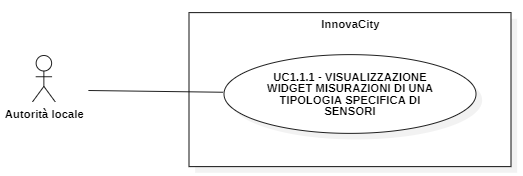
\includegraphics[width=0.9\textwidth]{../Images/uc1.1.1.png}
    \caption{UC1.1.1 - VISUALIZZAZIONE WIDGET MISURAZIONI DI UNA TIPOLOGIA SPECIFICA DI SENSORI }
    \label{fig:UC3}
\end{figure}

%---------------------------- UC1.1.1 ---------------------------------

\subsubsection{UC1.1.1 - VISUALIZZAZIONE WIDGET MISURAZIONI DI UNA TIPOLOGIA SPECIFICA DI SENSORI}

\begin{itemize}
    \item \textbf{Attore principale:} Autorità locale;
    \item \textbf{Precondizioni:}
        \begin{itemize}
            \item Il sistema è operativo e accessibile.
        \end{itemize}
    \item \textbf{Postcondizioni:}
        \begin{itemize}
            \item L'autorità locale visualizza uno specifico widget contenente le misurazioni rilevate da una specifica tipologia di sensori.
        \end{itemize}
    \item \textbf{Scenario principale:}
        \begin{enumerate}
            \item Il sistema ha caricato la visualizzazione della dashboard (UC1).
            \item Il sistema carica i dati e imposta la visualizzazione di uno specifico widget contenente le misurazioni relative ad una specifica tipologia di sensori.
        \end{enumerate}
    \item \textbf{User story associata:} \\
        Come autorità locale, voglio accedere a un widget dettagliato che rappresenti le misurazioni provenienti da una specifica tipologia di sensori. Questo mi permetterà di analizzare in modo approfondito i dati relativi a quella tipologia di sensori, aiutandomi a prendere decisioni mirate per migliorare i servizi della città.
\end{itemize}

%---------------------------- SUB_UC1.1.1 ---------------------------------

\begin{figure}[H]
    \centering
    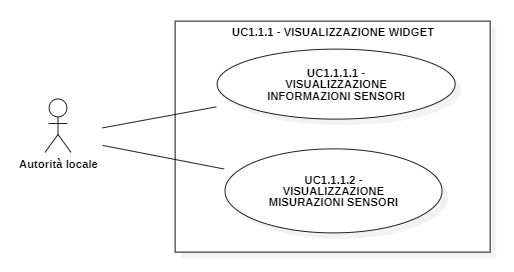
\includegraphics[width=0.9\textwidth]{../Images/subUC1.1.1.PNG}
    \caption{Sottocasi UC1.1.1 - VISUALIZZAZIONE WIDGET MISURAZIONI DI UNA TIPOLOGIA SPECIFICA DI SENSORI }
    \label{fig:UC3_sub}
\end{figure}

%---------------------------- UC1.1.1.1 ---------------------------------

\subsubsection{UC1.1.1.1 - VISUALIZZAZIONE INFORMAZIONI SENSORI}
\begin{itemize}
    \item \textbf{Attore principale:} Autorità locale;
    \item \textbf{Precondizioni:}
        \begin{itemize}
            \item Il \textit{sistema}\textsubscript{\textit{G}} è operativo e accessibile.
        \end{itemize}
    \item \textbf{Postcondizioni:}
        \begin{itemize}
            \item L’autorità locale ha una visione dettagliata sugli identificativi dei sensori che contribuiscono alle misurazioni rappresentate nel \textit{widget}\textsubscript{\textit{G}}.
        \end{itemize}
    \item \textbf{Scenario principale:}
        \begin{enumerate}
            \item Il \textit{sistema}\textsubscript{\textit{G}} carica e configura la visualizzazione di un \textit{widget}\textsubscript{\textit{G}} di una specifica tipologia di sensori (UC1.1.1);
            \item Il \textit{sistema}\textsubscript{\textit{G}} carica e configura la visualizzazione all'interno del \textit{widget}\textsubscript{\textit{G}} delle informazioni dei sensori coinvolti.
        \end{enumerate}
    \item \textbf{User story associata:} \\
        Come autorità locale, desidero visualizzare gli identificativi dei sensori associati alle misurazioni presentate nel \textit{widget}\textsubscript{\textit{G}}. Questo mi consentirà di comprendere meglio l'origine delle informazioni e facilitare la gestione e l'interpretazione dei dati raccolti.
\end{itemize}



%---------------------------- UC1.1.1.2 ---------------------------------

\subsubsection{UC1.1.1.2 - VISUALIZZAZIONE MISURAZIONI SENSORI}
\begin{itemize}
    \item \textbf{Attore principale:} Autorità locale;
    \item \textbf{Precondizioni:}
        \begin{itemize}
            \item Il \textit{sistema}\textsubscript{\textit{G}} è operativo e accessibile.
        \end{itemize}
    \item \textbf{Postcondizioni:}
        \begin{itemize}
            \item  L'autorità locale visualizza le misurazioni dei sensori associati al \textit{widget}\textsubscript{\textit{G}}.
        \end{itemize}
    \item \textbf{Scenario principale:}
        \begin{enumerate}
            \item Il \textit{sistema}\textsubscript{\textit{G}} carica e configura la visualizzazione di un \textit{widget}\textsubscript{\textit{G}} di una specifica tipologia di sensori (UC1.1.1);
            \item Il \textit{sistema}\textsubscript{\textit{G}} carica e configura la visualizzazione all'interno del \textit{widget}\textsubscript{\textit{G}} delle misurazioni dei sensori coinvolti.
        \end{enumerate}
    \item \textbf{User story associata:} \\
        Come autorità locale, desidero visualizzare le misurazioni dei sensori di una specifica tipologia per poter effettuare analisi mirate e prendere decisioni informate in base ai dati raccolti.
\end{itemize}


\begin{figure}[H]
    \centering
    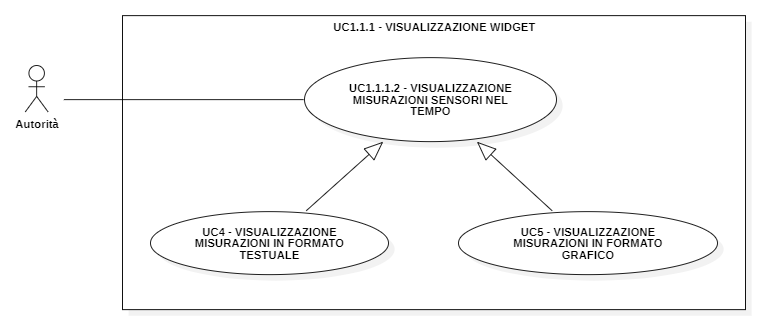
\includegraphics[width=0.9\textwidth]{../Images/uc1.1.1.2Gen.PNG}
    \caption{Generalizzazione UC1.1.1.2 - VISUALIZZAZIONE MISURAZIONI SENSORI }
    \label{fig:UC3_gen}
\end{figure}

\newpage

%---------------------------- UC4 ---------------------------------

\subsubsection{UC4 - Visualizzazione storico dati in formato testuale}
\begin{itemize}
    \item \textbf{Attore principale:} Autorità locale;
    \item \textbf{Descrizione:} L’autorità locale seleziona i/il sensore/i della quale vuole visionare lo storico dei dati e imposta la visulizzazione in formato testuale: (TIMESTAMP, Dato).
    \item \textbf{Scenario principale:}
          \begin{enumerate}
              \item L'utente imposta la visualizzazione in formato testuale.
          \end{enumerate}
    \item \textbf{Precondizioni:}
          \begin{itemize}
              \item  I/Il sensori/e di cui si vogliono visualizzare i dati storici ha trasmesso dati;
              \item  L'utente si trova in un interfaccia per la visualizzazione di uno storico dati (UC3).
          \end{itemize}
    \item \textbf{Postcondizioni:}
          \begin{itemize}
              \item  L'utente ha una visione dello storico dei dati trasmessi nel formato (TIMESTAMP, dato).
          \end{itemize}
    \item \textbf{User story associata:}
          \begin{itemize}
              \item Come autorità locale,
                    desidero visualizzare lo storico dei dati in formato testuale (TIMESTAMP, Dato),
                    In modo da avere una visione dettagliata delle informazioni trasmesse dai sensori.
          \end{itemize}
\end{itemize}

%---------------------------- UC5 ---------------------------------

\subsubsection{UC5 - VISUALIZZAZIONE MISURAZIONI IN FORMATO GRAFICO \newline TIME SERIES}
\begin{itemize}
    \item \textbf{Attore principale:} Autorità locale;
    \item \textbf{Precondizioni:}
        \begin{itemize}
            \item Il sistema è operativo e accessibile.
        \end{itemize}
    \item \textbf{Postcondizioni:}
        \begin{itemize}
            \item L'utente visualizza le misurazioni associate al widget attraverso un grafico time series.
        \end{itemize}
    \vspace{1cm}
    \item \textbf{Scenario principale:}
        \begin{enumerate}
            \item Il sistema carica e configura la visualizzazione di un widget di una specifica tipologia di sensori (UC1.1.1);
                \item Il sistema carica e configura la visualizzazione all'interno del widget delle misurazioni dei sensori coinvolti;
                \item L'autorità locale seleziona la visualizzazione delle misurazioni associato al widget in formato grafico.
        \end{enumerate}
    \item \textbf{User story associata:} \\
        Come autorità locale, desidero visualizzare le misurazioni associate ad uno specifico widget attraverso un grafico time series. Questo consente di semplificare la comprensione e la comparazione delle misurazioni, permettendo di individuare tendenze, relazioni e pattern in modo chiaro e rapido.
\end{itemize}
%---------------------------- UC14 ---------------------------------

\subsubsection{UC14 - VISUALIZZAZIONE MISURAZIONI IN FORMATO MAPPA INTERATTIVA}
\begin{itemize}
    \item \textbf{Attore principale:} Autorità locale;
    \item \textbf{Precondizioni:}
        \begin{itemize}
            \item Il sistema è operativo e accessibile.
        \end{itemize}
    \item \textbf{Postcondizioni:}
        \begin{itemize}
            \item L'utente visualizza le misurazioni correlate al widget mediante una mappa interattiva, la quale espone, attraverso apposite etichette, l'ultima rilevazione effettuata da ciascun sensore sulla mappa.
        \end{itemize}
    \item \textbf{Scenario principale:}
        \begin{enumerate}
            \item Il sistema carica e configura la visualizzazione di un widget di una specifica tipologia di sensori (UC1.1.1);
                \item Il sistema carica e configura la visualizzazione all'interno del widget delle misurazioni dei sensori coinvolti;
                \item Il widget è associato a sensori che generano dati binari (ex. Occupato / Libero, In funzione / Guasto).
              %  \item L'autorità locale seleziona la visualizzazione delle misurazioni associato al widget in formato mappa interattiva.
        \end{enumerate}
    \item \textbf{User story associata:} \\
        Come autorità locale, desidero poter visualizzare in modo chiaro e intuitivo le ultime rilevazioni effettuate da ciascun sensore associato al widget tramite una mappa interattiva, la quale, mediante etichette appropriate, rappresenti il valore della ultima misurazione effettuata da ciascun sensore.
\end{itemize}

%---------------------------- UC2 ---------------------------------
\begin{figure}[H]
    \centering
    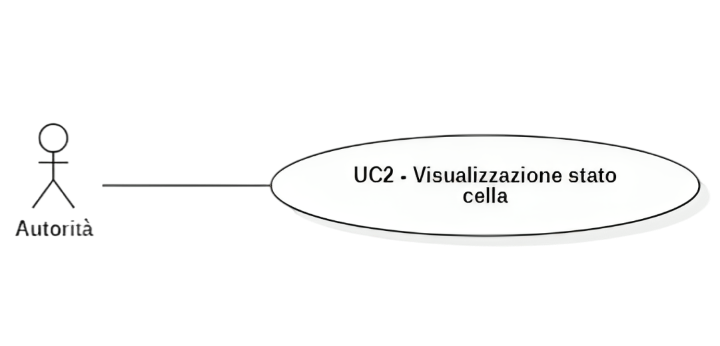
\includegraphics[width=0.9\textwidth]{../Images/uc2.png}
    \caption{UC2 - FILTRO VISUALIZZAZIONE DASHBOARD CELLA }
    \label{fig:UC2}
\end{figure}

\subsubsection{UC2 - Visualizzazione stato cella}
\begin{itemize}
    \item \textbf{Attore principale:} Autorità locale.
    \item \textbf{Descrizione:} L'autorità locale effettua la selezione della cella, ossia la specifica zona urbana, al fine di visualizzare in tempo reale i dati provenienti da varie tipologie di sensori ubicati nella suddetta area. Ciò permette una valutazione reapida dello stato complessivo della cella.
    \item \textbf{Scenario principale:}
        \begin{enumerate}
            \item L'utente seleziona la cella per la quale desidera visualizzare la dashboard contenente esclusivamente i dati correlati a essa.
        \end{enumerate}
    \item \textbf{Precondizioni:}
        \begin{itemize}
            \item  Almeno un sensore presente nella cella ha trasmesso dati;
            \item L'utente si trova  nella piattaforma per la visualizzazione della dashboard sullo stato della città (UC1);
        \end{itemize}
    \item \textbf{Postcondizioni:}
        \begin{itemize}
            \item  L'utente ha una visione aggiornata dello stato di salute della cella tramite widget e grafici interattivi aggiornati in tempo reale sulla base di dati correlati esclusivamente alla cella, inoltre visualizza una mappa dei sensori presenti nella cella e un punteggio di salute relativo alla cella.
          \end{itemize}
    \item \textbf{User story associata:}
        \begin{itemize}
            \item Come autorità locale, desidero poter selezionare una specifica cella urbana sulla piattaforma al fine di visualizzare immediatamente i dati provenienti da vari sensori presenti nell'area. Questo mi permetterà di valutare rapidamente lo stato complessivo della cella e prendere decisioni informate.
        \end{itemize}
\end{itemize}

%---------------------------- UC6 ---------------------------------

\begin{figure}[H]
    \centering
    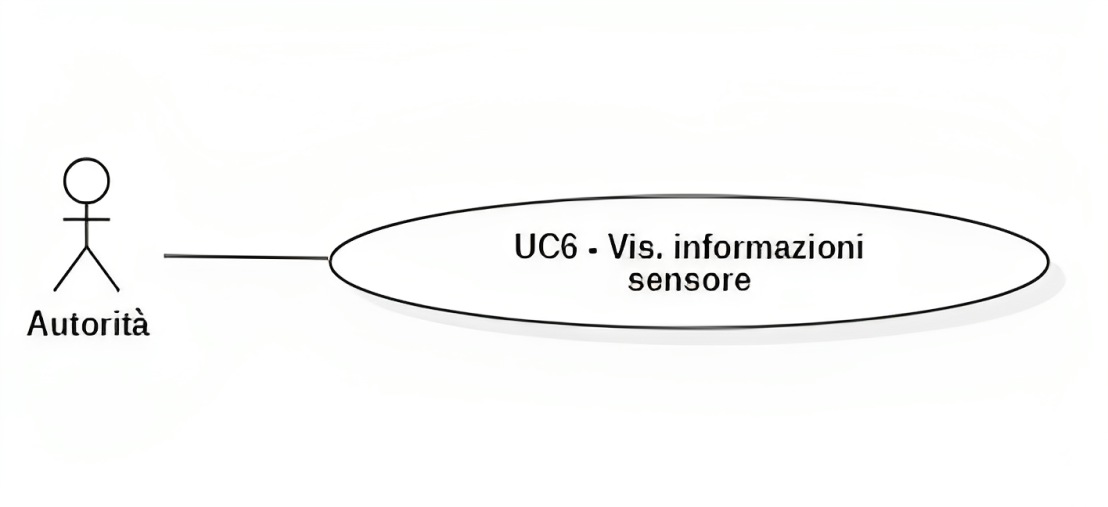
\includegraphics[width=0.9\textwidth]{../Images/uc6.png}
    \caption{UC6 - VISUALIZZAZIONE WIDGET SENSORI TEMPERATURA }
    \label{fig:UC6}
\end{figure}

\subsubsection{UC6 - VISUALIZZAZIONE WIDGET SENSORI TEMPERATURA}
\begin{itemize}
    \item \textbf{Attore principale:} Autorità locale;
    \item \textbf{Precondizioni:}
        \begin{itemize}
            \item Almeno un sensore di temperatura ha trasmesso dati al sistema;
            \item Il sistema ha caricato la visualizzazione della dashboard (UC1).
        \end{itemize}
    \item \textbf{Postcondizioni:}
        \begin{itemize}
            \item L'autorità locale visualizza un widget contenente le misurazioni relative ai sensori di temperatura.
        \end{itemize}
    \item \textbf{Scenario principale:}
        \begin{enumerate}
            \item Il sistema carica i dati e imposta la visualizzazione del widget contenente le misurazioni relative ai sensori di temperatura.
        \end{enumerate}
    \item \textbf{User story associata:} \\
        Come autorità locale, desidero visualizzare un widget per la visualizzazione delle misurazioni trasmesse dai sensori di temperatura. Questo mi permetterà di analizzare in modo approfondito i dati relativi a quella tipologia di sensori, aiutandomi a prendere decisioni mirate per migliorare i servizi della città.
\end{itemize}

%---------------------------- UC7 ---------------------------------

\begin{figure}[H]
    \centering
    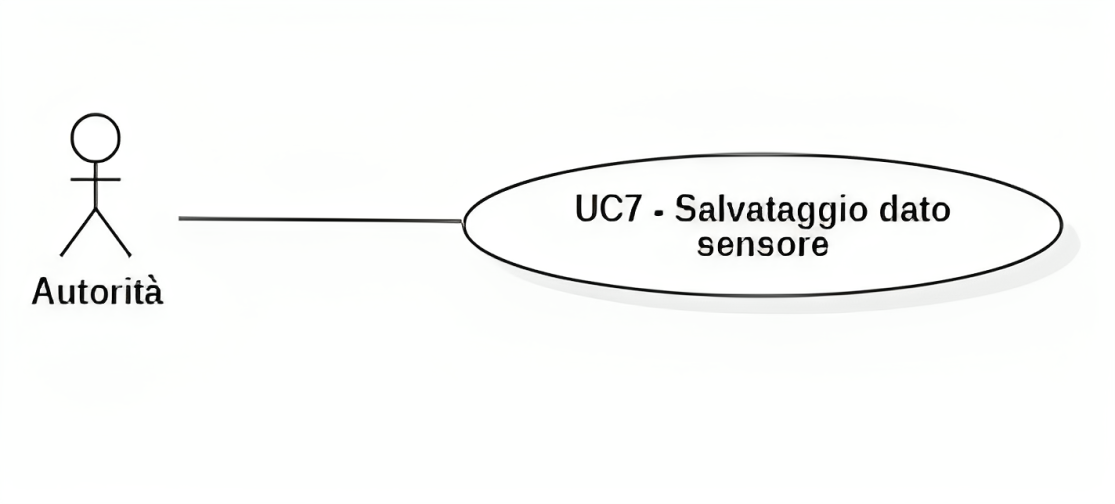
\includegraphics[width=0.9\textwidth]{../Images/uc7.png}
    \caption{UC7 - VISUALIZZAZIONE WIDGET SENSORI UMIDITÀ }
\end{figure}

\subsubsection{UC7 - VISUALIZZAZIONE WIDGET SENSORI UMIDITÀ}
\begin{itemize}
    \item \textbf{Attore principale:} Autorità locale;
    \item \textbf{Precondizioni:}
        \begin{itemize}
            \item Il sistema ha caricato la visualizzazione della dashboard (UC1).
        \end{itemize}
    \item \textbf{Postcondizioni:}
        \begin{itemize}
            \item L'autorità locale visualizza un widget contenente le misurazioni relative ai sensori di umidità.
        \end{itemize}
    \item \textbf{Scenario principale:}
        \begin{enumerate}
            \item Il sistema carica i dati e imposta la visualizzazione del widget contenente le misurazioni relative ai sensori di umidità.
        \end{enumerate}
    \item \textbf{User story associata:} \\
        Come autorità locale, desidero visualizzare un widget per la visualizzazione delle misurazioni trasmesse dai sensori di umidità. Questo mi permetterà di analizzare in modo approfondito i dati relativi a quella tipologia di sensori, aiutandomi a prendere decisioni mirate per migliorare i servizi della città.
\end{itemize}

%---------------------------- UC8 ---------------------------------

\begin{figure}[H]
    \centering
    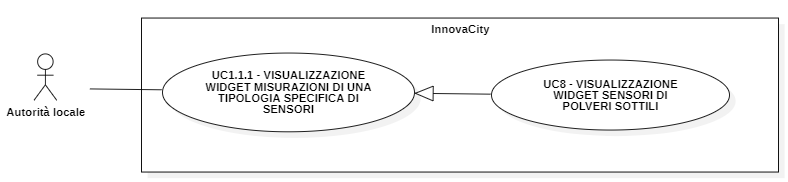
\includegraphics[width=0.9\textwidth]{../Images/uc8.PNG}
    \caption{UC8 - VISUALIZZAZIONE WIDGET SENSORI DI POLVERI SOTTILI }
\end{figure}

\subsubsection{UC8 - VISUALIZZAZIONE WIDGET SENSORI DI POLVERI SOTTILI}
\begin{itemize}
    \item \textbf{Attore principale:} Autorità locale;
    %\item \textbf{Descrizione:} L’autorità locale dalla pagina adibita alla visione dello storico dati di un sensore seleziona la visualizzazione delle informazioni sul sensore.
    \item \textbf{Scenario principale:}
          \begin{enumerate}
              \item L'autorità locale seleziona la visualizzazione del widget dei sensori di polveri sottili.
          \end{enumerate}
    \item \textbf{Precondizioni:}
          \begin{itemize}
              \item  Almeno un sensore di polveri sottili ha trasmesso dati al sistema.
          \end{itemize}
    \item \textbf{Postcondizioni:}
          \begin{itemize}
              \item  L'autorità locale ha una visione di un widget contenente le informazioni dei sensori di polveri sottili.
          \end{itemize}
    \item \textbf{User story associata:}
          \begin{itemize}
              \item Come Autorità locale, desidero visualizzare un widget per la visualizzazione delle misurazione dei sensori di polveri sottili.
          \end{itemize}
\end{itemize}

%---------------------------- UC9 ---------------------------------
\begin{figure}[H]
    \centering
    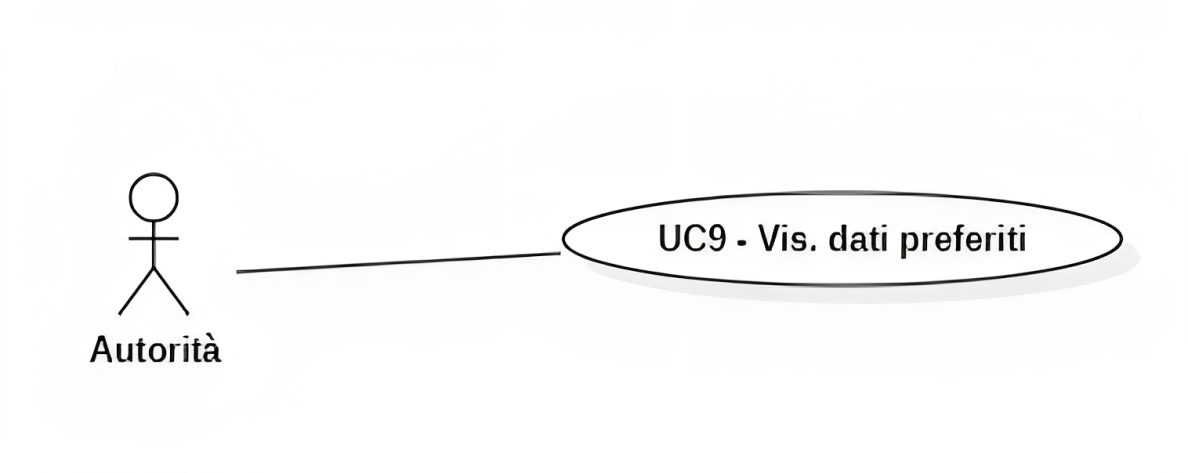
\includegraphics[width=0.9\textwidth]{../Images/uc9.png}
    \caption{UC9 - VISUALIZZAZIONE WIDGET SENSORI DI GUASTI ELETTRICI }
\end{figure}

\subsubsection{UC9 - Visualizzazione dati preferiti}
\begin{itemize}
    \item \textbf{Attore principale:} Autorità locale;
    \item \textbf{Descrizione:} L’autorità locale seleziona la visulizzazione dei dati preferiti.
    \item \textbf{Scenario principale:}
          \begin{enumerate}
              \item L'utente accede alla piattaforma per la visualizzazione della dashboard sullo stato della città o di una cella(UC1) (UC1.1);
              \item L'utente sceglie di visualizzare la pagina dedicata alla visualizzazione dei dati preferiti.
          \end{enumerate}
    \item \textbf{Precondizioni:}
          \begin{itemize}
              \item  L'utente si trova nella pagina per la visualizzazione delle dashboard (UC1) (UC1.1);
          \end{itemize}
    \item \textbf{Postcondizioni:}
          \begin{itemize}
              \item  L'utente ha una visione dei dati dei sensori salvati come preferiti.
          \end{itemize}
    \item \textbf{User story associata:}
          \begin{itemize}
              \item Come di Autorità Locale, desidero visualizzare i dati dei sensori precedentemente salvati come preferiti sulla piattaforma, così da poter accedere rapidamente alle informazioni rilevanti.
          \end{itemize}
\end{itemize}
%---------------------------- UC10 ---------------------------------
\newpage

\begin{figure}[H]
    \centering
    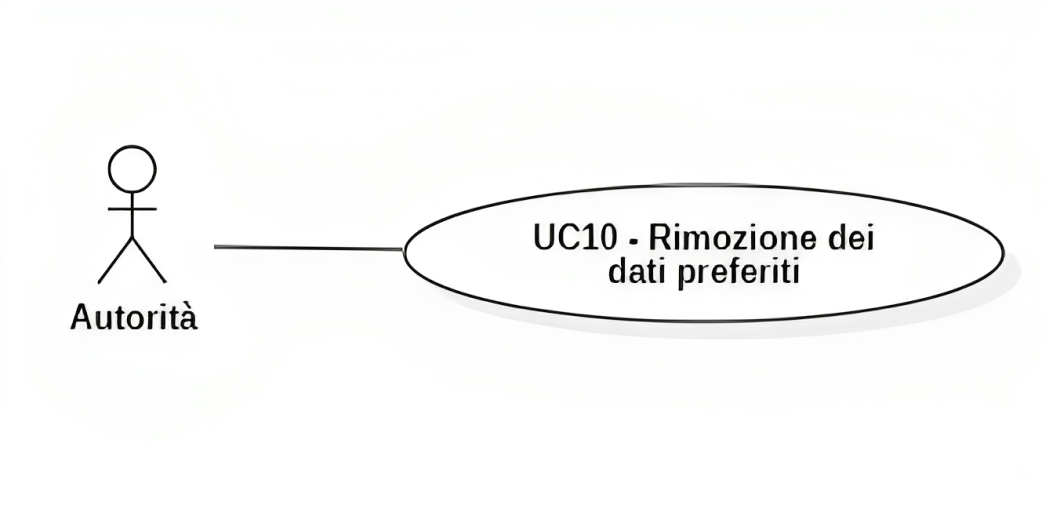
\includegraphics[width=0.9\textwidth]{../Images/uc10.png}
    \caption{UC10 - VISUALIZZAZIONE WIDGET SENSORI ISOLE ECOLOGICHE }
\end{figure}

\subsubsection{UC10 - VISUALIZZAZIONE WIDGET SENSORI ISOLE ECOLOGICHE}
\begin{itemize}
    \item \textbf{Attore principale:} Autorità locale;
    \item \textbf{Precondizioni:}
        \begin{itemize}
            \item Almeno un sensore di rilevamento soglia delle isole ecologiche ha trasmesso dati al sistema;
            \item Il sistema ha caricato la visualizzazione della dashboard (UC1).
        \end{itemize}
    \item \textbf{Postcondizioni:}
        \begin{itemize}
            \item L'autorità locale visualizza un widget contenente le misurazioni relative ai sensori di rilevamento soglia delle isole ecologiche.
        \end{itemize}
    \item \textbf{Scenario principale:}
        \begin{enumerate}
            \item Il sistema carica i dati e imposta la visualizzazione del widget contenente le misurazioni relative ai sensori di rilevamento soglia delle isole ecologiche.
        \end{enumerate}
    \item \textbf{User story associata:} \\
        Come autorità locale, desidero visualizzare un widget per la visualizzazione delle misurazioni trasmesse dai sensori di rilevamento soglia delle isole ecologiche. Questo mi permetterà di analizzare in modo approfondito i dati relativi a quella tipologia di sensori, aiutandomi a prendere decisioni mirate per migliorare i servizi della città.
\end{itemize}
%---------------------------- UC11 ---------------------------------
\begin{figure}[H]
    \centering
    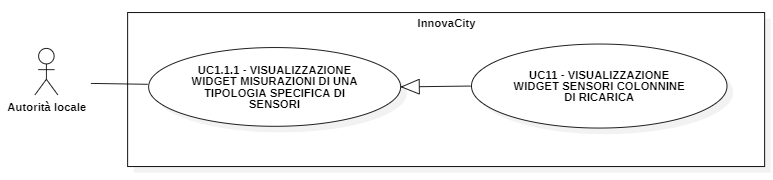
\includegraphics[width=0.9\textwidth]{../Images/uc11.PNG}
    \caption{UC11 - VISUALIZZAZIONE WIDGET SENSORI COLONNINE DI RICARICA }
\end{figure}

\subsubsection{UC11 - Visualizzazione storico dati in ordine crescente}
\begin{itemize}
    \item \textbf{Attore principale:} Autorità locale;
    \item \textbf{Descrizione:} L’autorità locale seleziona i/il sensore/i della quale vuole visionare lo storico dei dati in formato testuale in ordine crescente rispetto alle misurazioni del/i sensore/i.
    \item \textbf{Scenario principale:}
          \begin{enumerate}
              \item L'utente imposta la visualizzazione in ordine crescente.
          \end{enumerate}
    \item \textbf{Precondizioni:}
          \begin{itemize}
              \item  I/Il sensori/e di cui si vuole visualizzare i dati storici ha trasmesso dati;
              \item  L'utente si trova in un interfaccia per la visualizzazione di uno storico dati (UC3);
              \item La visualizzazione è impostata nel formato testuale (UC4);
          \end{itemize}
    \item \textbf{Postcondizioni:}
          \begin{itemize}
              \item  L'utente ha una visione dello storico dei dati trasmessi nel formato (TIMESTAMP, dato) in ordine crescente rispetto alle misurazioni.
          \end{itemize}
    \item \textbf{User story associata:}
          \begin{itemize}
              \item Come autorità locale, desidero essere in grado di visualizzare lo storico dei dati provenienti dai sensori in formato testuale, ordinati in modo crescente rispetto alla misurazione del/i sensore/i, al fine di identificare facilmente tendenze, cambiamenti o pattern nel tempo.
          \end{itemize}
\end{itemize}

%---------------------------- UC33 ---------------------------------

\begin{figure}[H]
    \centering
    \includegraphics[width=0.9\textwidth]{../Images/uc33.PNG}
    \caption{UC33 - VISUALIZZAZIONE WIDGET SENSORI LIVELLO DELL'ACQUA }
\end{figure}

\subsubsection{UC33 - VISUALIZZAZIONE WIDGET SENSORI LIVELLO DELL'ACQUA}
\begin{itemize}
    \item \textbf{Attore principale:} Autorità locale;
    \item \textbf{Precondizioni:}
        \begin{itemize}
            \item Almeno un sensore del livello dell'acqua ha trasmesso dati al sistema;
            \item Il sistema ha caricato la visualizzazione della dashboard (UC1).
        \end{itemize}
    \item \textbf{Postcondizioni:}
        \begin{itemize}
            \item L'autorità locale visualizza un widget contenente le misurazioni relative ai sensori del livello dell'acqua.
        \end{itemize}
    \item \textbf{Scenario principale:}
        \begin{enumerate}
            \item Il sistema carica i dati e imposta la visualizzazione del widget contenente le misurazioni relative ai sensori del livello dell'acqua.
        \end{enumerate}
    \item \textbf{User story associata:} \\
        Come autorità locale, desidero visualizzare un widget per la visualizzazione delle misurazioni trasmesse dai sensori del livello dell'acqua. Questo mi permetterà di analizzare in modo approfondito i dati relativi a quella tipologia di sensori, aiutandomi a prendere decisioni mirate per migliorare i servizi della città.
\end{itemize}

%---------------------------- UC12 ---------------------------------
\newpage

\begin{figure}[H]
    \centering
    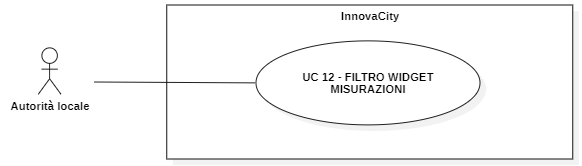
\includegraphics[width=0.9\textwidth]{../Images/uc12.PNG}
    \caption{UC 12 - FILTRO WIDGET MISURAZIONI }
\end{figure}

\subsubsection{UC12 - FILTRO WIDGET MISURAZIONI}
\begin{itemize}
    \item \textbf{Attore principale:} Autorità locale;
    \item \textbf{Precondizioni:}
        \begin{itemize}
            \item L'autorità locale si trova nell'interfaccia di visualizzazione di un \textit{widget}\textsubscript{\textit{G}} associato ad una specifica tipologia di sensori (UC1.1.1);
        \end{itemize}
    \item \textbf{Postcondizioni:}
          \begin{itemize}
              \item L'autorità locale visualizza esclusivamente le misurazioni che soddisfano il filtraggio.
          \end{itemize}
    \item \textbf{Scenario principale:}
          \begin{enumerate}
              \item L'utente seleziona i filtri da applicare;
              \item Il \textit{sistema}\textsubscript{\textit{G}} aggiorna la visualizzazione mostrando esclusivamente le misurazioni che rispettano i vincoli specificati filtri.
          \end{enumerate}
    \item \textbf{User story associata:} \\
        Come autorità locale, desidero disporre della capacità di applicare filtri per la visualizzazione delle misurazioni, consentendo un'analisi dettagliata e focalizzata attraverso una combinazione di criteri selettivi.
\end{itemize}


%---------------------------- UC12.1 ---------------------------------
\newpage

\begin{figure}[H]
    \centering
    \includegraphics[width=0.9\textwidth]{../Images/uc12.1.PNG}
    \caption{UC12.1 - FILTRO VISUALIZZAZIONE MISURAZIONI IN UN INTERVALLO TEMPORALE }
\end{figure}

\subsubsection{UC12.1 - FILTRO VISUALIZZAZIONE MISURAZIONI IN UN INTERVALLO TEMPORALE}
\begin{itemize}
    \item \textbf{Attore principale:} Autorità locale;
    \item \textbf{Precondizioni:}
        \begin{itemize}
            \item L'autorità locale si trova nell'interfaccia di visualizzazione di un \textit{widget}\textsubscript{\textit{G}} associato ad una specifica tipologia di sensori (UC1.1.1); 
            \item L'autorità locale ha impostato la vista in formato testuale time series o in formato grafico time series.
        \end{itemize}
    \item \textbf{Postcondizioni:}
        \begin{itemize}
            \item L'autorità locale visualizza le sole misurazioni trasmesse da una specifica tipolgia di sensori nell'intervallo temporale selezionato.
        \end{itemize}
    \item \textbf{Scenario principale:}
        \begin{enumerate}
            \item L'autorità locale seleziona la funzionalità relativa al filtro dei dati per intervallo temporale;
            \item L'autorità locale imposta un intervallo temporale;
            \item Il \textit{sistema}\textsubscript{\textit{G}} verifica la validità dell'intervallo temporale inserito;
            \item Il \textit{sistema}\textsubscript{\textit{G}} aggiorna la visualizzazione mostrando solo le misurazioni effettuate durante l'intervallo temporale. selezionato.
        \end{enumerate}
    \item \textbf{Estensioni:}
    \begin{enumerate}
        \item VISUALIZZAZIONE ERRORE INTERVALLO TEMPORALE NON VALIDO (UC30)
    \end{enumerate}
    \item \textbf{User story associata:} \\
        Come autorità locale, voglio avere la capacità di definire un intervallo temporale personalizzato per poter filtrare le misurazioni trasmesse da una specifica tipologia di sensori. Ciò mi permetterà di analizzare dettagliatamente le misurazioni raccolte in un periodo di interesse specifico.
\end{itemize}

%---------------------------- UC30 ---------------------------------
\subsubsection{UC30 - VISUALIZZAZIONE ERRORE INTERVALLO TEMPORALE NON VALIDO}
\begin{itemize}
      \item \textbf{Attore principale:} Autorità locale;
      \item \textbf{Precondizioni:}
            \begin{itemize} 
                  \item L'autorità locale specifica un intervallo temporale non valido per la visualizzazione filtrata delle misurazioni;
            \end{itemize}
            \item \textbf{Postcondizioni:}
            \begin{itemize}
                  \item L'autorità locale visualizza un messaggio di errore.
            \end{itemize}
            \item \textbf{Scenario principale:}
            \begin{enumerate}
                  \item Il sistema rileva l'invalidità dell'intervallo temporale specificato dall'autorità locale.
                  \end{enumerate}
      \item \textbf{User story associata:} \\
            Come autorità locale, desidero ricevere una notifica immediata nel caso in cui selezioni un intervallo temporale non valido come filtro per la visualizzazione delle misurazioni. Questo mi permetterà di ricevere un feedback istantaneo e mi darà la possibilità di inserire successivamente un intervallo temporale corretto.
\end{itemize}

%---------------------------- UC12.2 ---------------------------------

\begin{figure}[H]
    \centering
    \includegraphics[width=0.9\textwidth]{../Images/uc12.2.PNG}
    \caption{UC12.2 -FILTRO VISUALIZZAZIONE PER MISURAZIONI }
\end{figure}

\subsubsection{UC12.2 - FILTRO VISUALIZZAZIONE PER MISURAZIONI}
\begin{itemize}
    \item \textbf{Attore principale:} Autorità locale;
    \item \textbf{Precondizioni:}
        \begin{itemize}
            \item L'autorità locale si trova nell'interfaccia di visualizzazione di un widget associato ad una specifica tipologia di sensori (UC1.1.1);
            \item L'autorità locale ha impostato la vista in formato testuale Time series o in formato grafico Time Series.
        \end{itemize}
    \item \textbf{Postcondizioni:}
        \begin{itemize}
            \item L'utente visualizza le misurazioni filtrate includendo soltanto i dati rilevati che si collocano tra i due valori specificati.
        \end{itemize}
    \item \textbf{Scenario principale:}
        \begin{enumerate}
            \item L'autorità locale seleziona la funzionalità relativa al filtro dei dati per intervallo di rilevamento;
            \item L'utente inserisce un valore di minimo ed un valore di massimo per filtrare le misurazioni;
            \item Il sistema verifica la validità dell'intervallo di rilevamento inserito;
            \item Il sistema aggiorna la visualizzazione mostrando esclusivamente le misurazioni con il dato rilevato che ricade all'interno dell'intervallo specificato.
        \end{enumerate}
    \item \textbf{Estensioni:}
        \begin{enumerate}
            \item VISUALIZZAZIONE ERRORE INTERVALLO DI RILEVAMENTO NON VALIDO (UC32)
        \end{enumerate}
    \item \textbf{User story associata:} \\
        Come autorità locale, desidero avere la possibilità di visualizzare le misurazioni filtrate includendo soltanto i dati rilevati che si collocano tra un valore di minimo e di massimo specifici. Questo mi consentirà di analizzare in modo più mirato e focalizzato le misurazioni che rientrano in un determinato intervallo di rilevamento, facilitando l'identificazione di pattern o anomalie significative.
\end{itemize}


%---------------------------- UC32 ---------------------------------
\subsubsection{UC30 - VISUALIZZAZIONE ERRORE INTERVALLO DI RILEVAMENTO NON VALIDO}
\begin{itemize}
    \item \textbf{Attore principale:} Autorità locale;
    \item \textbf{Precondizioni:}
        \begin{itemize} 
            \item L'autorità locale specifica un intervallo di rilevamento non valido per la visualizzazione filtrata delle misurazioni;
            \item Il sistema rileva l'invalidità dell'intervallo di rilevamento specificato dall'autorità locale.
        \end{itemize}
    \item \textbf{Postcondizioni:}
        \begin{itemize}
            \item L'autorità locale visualizza un messaggio di errore e viene richiesto l'inserimento di un nuovo intervallo di rilevamento.
        \end{itemize}
    \item \textbf{Scenario principale:}
            \begin{enumerate}
            \item L'autorità locale visualizza di un messaggio di errore;
            \item Il sistema richiede all'autorità locale di inserire un intervallo di rilevamento valido.
            \end{enumerate}
    \item \textbf{User story associata:}
        Come autorità locale, desidero ricevere una notifica immediata nel caso in cui selezioni un intervallo di rilevamento non valido come filtro per la visualizzazione delle misurazioni. Questo mi permetterà di ricevere un feedback istantaneo e mi darà la possibilità di inserire successivamente un intervallo di rilevamento corretto.
\end{itemize}

%---------------------------- UC12.3 ---------------------------------
\newpage

\begin{figure}[H]
    \centering
    \includegraphics[width=0.9\textwidth]{../Images/uc12.3.PNG}
    \caption{UC12.3 - FILTRO VISUALIZZAZIONE MISURAZIONI PER CELLA }
\end{figure}

\subsubsection{UC12.3 - FILTRO VISUALIZZAZIONE MISURAZIONI PER CELLA}
\begin{itemize}
    \item \textbf{Attore principale:} Autorità locale;
    \item \textbf{Precondizioni:}
        \begin{itemize}
            \item L'autorità locale si trova nell'interfaccia di visualizzazione di un widget associato ad una specifica tipologia di sensori (UC1.1.1);
            \item Almeno una cella urbana è presente nella città. 
        \end{itemize}
    \item \textbf{Postcondizioni:}
          \begin{itemize}
              \item L'autorità locale visualizza esclusivamente le misurazioni trasmesse dai sensori di una o più specifiche celle selezionate.
          \end{itemize}
    \item \textbf{Scenario principale:}
          \begin{enumerate}
              \item L'autorità locale seleziona la funzionalità relativa al filtro per cella urbana;
              \item L'autorità locale seleziona una o più celle come filtro;
              \item Il sistema aggiorna la visualizzazione mostrando esclusivamente le misurazioni dei sensori all'interno delle celle urbane selezionate.
          \end{enumerate}
    \item \textbf{User story associata:} \\
        Come autorità locale, desidero poter filtrare la visualizzazione delle misurazioni in base alle singole celle urbane, consentendo un'esplorazione dettagliata dei dati rilevanti per ciascuna area della città.
\end{itemize}

%---------------------------- UC12.4 ---------------------------------
\begin{figure}[H]
    \centering
    \includegraphics[width=0.9\textwidth]{../Images/uc12.4.PNG}
    \caption{UC12.4 - FILTRO VISUALIZZAZIONE MISURAZIONI PER SENSORE }
\end{figure}
\subsubsection{UC12.4 - FILTRO VISUALIZZAZIONE MISURAZIONI PER SENSORE}
\begin{itemize}
    \item \textbf{Attore principale:} Autorità locale;
    \item \textbf{Precondizioni:}
        \begin{itemize}
            \item L'autorità locale si trova nell'interfaccia di visualizzazione di un widget associato ad una specifica tipologia di sensori (UC1.1.1);
        \end{itemize}
    \item \textbf{Postcondizioni:}
        \begin{itemize}
            \item L'autorità locale visualizza esclusivamente le misurazioni trasmesse da uno o più specifici sensori selezionati.
        \end{itemize}
    \item \textbf{Scenario principale:}
        \begin{enumerate}
            \item L'autorità locale seleziona la funzionalità relativa al filtro per sensore;
            \item L'autorità locale seleziona uno o più sensori come filtro;
            \item Il sistema aggiorna la visualizzazione mostrando esclusivamente le misurazioni tramsesse dai sensori selezionati.
        \end{enumerate}
    \item \textbf{User story associata:} \\
        Come autorità locale, desidero filtrare la visualizzazione delle misurazioni in base ad una selezione di specifici sensori, permettendo un'analisi dettagliata e specifica per ciascun sensore presenti nella città.
\end{itemize}


%---------------------------- UC13 ---------------------------------

\begin{figure}[H]
    \centering
    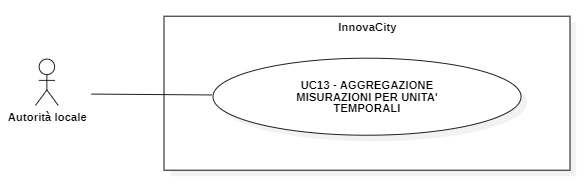
\includegraphics[width=0.9\textwidth]{../Images/uc13.PNG}
    \caption{UC13 - AGGREGAZIONE MISURAZIONI PER UNITA' TEMPORALI }
\end{figure}

\subsubsection{UC13 - Visualizzazione storico dati filtrato sulle misurazioni}
\begin{itemize}
    \item \textbf{Attore principale:} Autorità locale;
    \item \textbf{Descrizione:} L’autorità locale seleziona i/il sensore/i della quale vuole visionare lo storico dei dati e filtra la visualizzazione ai soli dati compresi tra due valori.
    \item \textbf{Scenario principale:}
          \begin{enumerate}
              \item L'utente configura due valori specifici al fine di visualizzare esclusivamente le misurazioni che ricadono all'interno di tale intervallo.
          \end{enumerate}
    \item \textbf{Precondizioni:}
          \begin{itemize}
              \item  I/Il sensori/e di cui si vuole visualizzare i dati storici ha trasmesso dati;
              \item  L'utente si trova in un interfaccia per la visualizzazione di uno storico dati (UC3).
          \end{itemize}
    \item \textbf{Postcondizioni:}
          \begin{itemize}
              \item  L'utente accede a una rappresentazione dello storico dei dati trasmessi, la cui visualizzazione è stata filtrata esclusivamente per includere le misurazioni con il dato compreso tra i due valori specificati.
          \end{itemize}
    \item \textbf{User story associata:}
          \begin{itemize}
            \item Come autorità locale, desidero avere la possibilità di filtrare la visualizzazione dello storico dei dati in base alle misurazioni del sensore comprese tra due valori specifici. Questo mi consentirà di analizzare in modo più mirato e focalizzato i dati che rientrano in un determinato intervallo, facilitando l'identificazione di pattern o anomalie significative.
          \end{itemize}
\end{itemize}


%---------------------------- UC31 ---------------------------------

\begin{figure}[H]
    \centering
    \includegraphics[width=0.9\textwidth]{../Images/uc31.PNG}
    \caption{UC31 - RIMOZIONE FILTRI }
    \label{fig:UC7}
\end{figure}
\subsubsection{UC31 - RIMOZIONE FILTRI}
\begin{itemize}
    \item \textbf{Attore principale:} Autorità locale;
    \item \textbf{Precondizioni:}
        \begin{itemize}
        \item L'autorità locale si trova nell'interfaccia di visualizzazione di un widget associato ad una specifica tipologia di sensori (UC1.1.1);
        \item La visualizzazione delle misurazioni include almeno un filtro attivo.
        \end{itemize}
    \item \textbf{Postcondizioni:}
        \begin{itemize}
            \item L'autorità locale visualizza le misurazioni senza nessun filtro applicato.
        \end{itemize}
    \item \textbf{Scenario principale:}
        \begin{enumerate}
            \item L'utente rimuove uno o più filtri relativi alle misurazioni.
            \item Il sistema aggiorna la visualizzazione senza l'applicazione dei filtri disattivati.
        \end{enumerate}
    \item \textbf{User story associata:} \\
        Come autorità locale, desidero rimuovere eventuali filtri attivi nella visualizzazione delle misurazioni in modo tale da tornare alla visualizzazione delle misurazioni senza tali filtri.
\end{itemize}


%---------------------------- UC18 ---------------------------------

\begin{figure}[H]
    \centering
    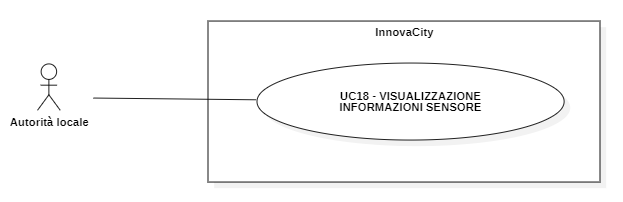
\includegraphics[width=0.9\textwidth]{../Images/uc18.PNG}
    \caption{UC18 - VISUALIZZAZIONE INFORMAZIONI SENSORE }
\end{figure}
\subsubsection{UC18 - VISUALIZZAZIONE INFORMAZIONI SENSORE}
\begin{itemize}
    \item \textbf{Attore principale:} Autorità locale;
    \item \textbf{Precondizioni:}
        \begin{itemize}
            \item Il sistema ha caricato la visualizzazione della dashboard (UC1);
        \end{itemize}
    \item \textbf{Postcondizioni:}
        \begin{itemize}
            \item L'autorità locale visualizza le informazioni relative ad uno specifico sensore.
        \end{itemize}
    \item \textbf{Scenario principale:}
        \begin{enumerate}
            \item L'autorità locale seleziona un sensore dalla mappa interattiva della città presente nella dashboard;
            \item Il sistema carica le informazioni relative al sensore selezionato.
        \end{enumerate}
    \item \textbf{User story associata:} \\
        Come autorità locale, desidero accedere alle informazioni dettagliate di un sensore specifico per ottenere una comprensione esaustiva delle sue caratteristiche e specifiche.
\end{itemize}

%---------------------------- SUB_UC18 ---------------------------------

\begin{figure}[H]
    \centering
    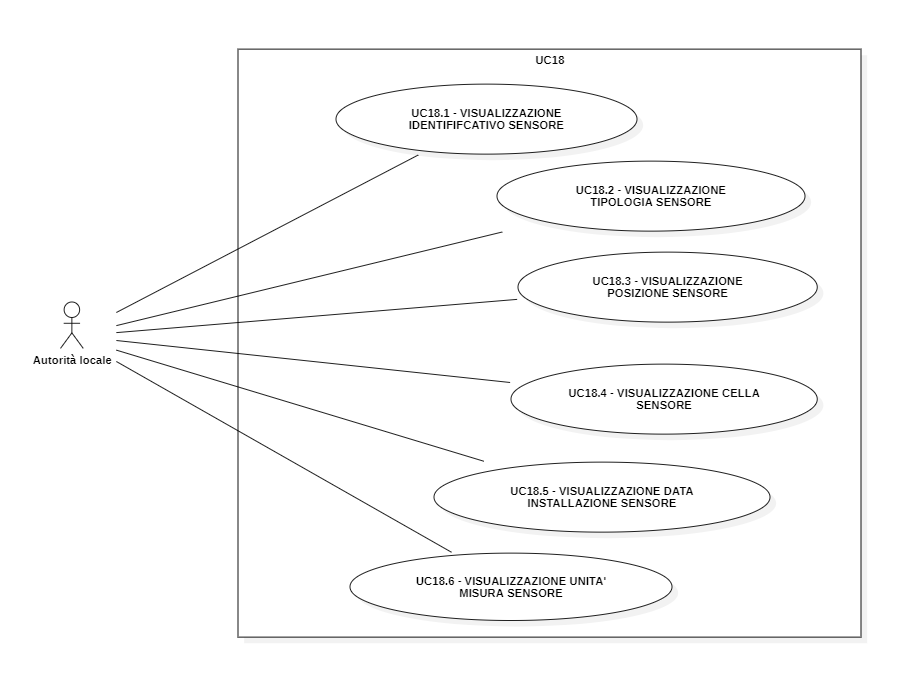
\includegraphics[width=0.9\textwidth]{../Images/uc18sub.PNG}
    \caption{SOTTOCASI UC18 - VISUALIZZAZIONE INFORMAZIONI SENSORE }
\end{figure}

%---------------------------- UC18.1 ---------------------------------

\subsubsection{UC18.1 - VISUALIZZAZIONE IDENTIFICATIVO SENSORE}
\begin{itemize}
    \item \textbf{Attore principale:} Autorità locale;
    %\item \textbf{Descrizione:} L’autorità locale dalla pagina adibita alla visione delle informazioni di un sensore visualizza il suo Identificativo.
    \item \textbf{Scenario principale:}
    \begin{enumerate}
        \item L'utente seleziona la visualizzazione delle informazioni del sensore.
    \end{enumerate}
\item \textbf{Precondizioni:}
    \begin{itemize}
        \item  L'utente di trova nella pagina di visualizzazione dello storico dei dati di un sensore. (3.3)
    \end{itemize}
    \item \textbf{Postcondizioni:}
          \begin{itemize}
              \item  L'utente visualizza l'Identificativo del sensore.
          \end{itemize}\item \textbf{User story associata:}
          \begin{itemize}
              \item Come Autorità Locale, desidero visualizzare l'identificativo di un sensore dalla pagina dedicata alle informazioni del sensore.
          \end{itemize}
\end{itemize}

%---------------------------- UC18.2 ---------------------------------

\subsubsection{UC18.2 - VISUALIZZAZIONE TIPOLOGIA SENSORE}
\begin{itemize}
    \item \textbf{Attore principale:} Autorità locale;
  %  \item \textbf{Descrizione:} L’autorità locale dalla pagina adibita alla visione delle informazioni di un sensore visualizza la sua tipologia (ex. Termometro).
    \item \textbf{Scenario principale:}
    \begin{enumerate}
        \item L'utente seleziona la visualizzazione delle informazioni del sensore.
    \end{enumerate}
\item \textbf{Precondizioni:}
    \begin{itemize}
        \item  L'utente di trova nella pagina di visualizzazione dello storico dei dati di un sensore. (3.3)
    \end{itemize}
    \item \textbf{Postcondizioni:}
          \begin{itemize}
              \item  L'utente visualizza la tipologia del sensore.
          \end{itemize}\item \textbf{User story associata:}
          \begin{itemize}
              \item Come Autorità Locale, desidero visualizzare la tipolgia di un sensore dalla pagina dedicata alle informazioni del sensore.
          \end{itemize}
\end{itemize}

%---------------------------- UC18.3 ---------------------------------

\subsubsection{UC18.3 - VISUALIZZAZIONE POSIZIONE SENSORE}
\begin{itemize}
    \item \textbf{Attore principale:} Autorità locale;
    %\item \textbf{Descrizione:} L’autorità locale dalla pagina adibita alla visione delle informazioni di un sensore visualizza la sua posizione in coordinate.
    \item \textbf{Scenario principale:}
    \begin{enumerate}
        \item L'utente seleziona la visualizzazione delle informazioni del sensore.
    \end{enumerate}
\item \textbf{Precondizioni:}
    \begin{itemize}
        \item  L'utente di trova nella pagina di visualizzazione dello storico dei dati di un sensore. (3.3)
    \end{itemize}
    \item \textbf{Postcondizioni:}
          \begin{itemize}
              \item  L'utente visualizza le coordinate del sensore.
          \end{itemize}
    \item \textbf{User story associata:}
          \begin{itemize}
              \item Come Autorità Locale, desidero visualizzare la posizione di un sensore, in coordinate, dalla pagina dedicata alle informazioni del sensore.
          \end{itemize}
\end{itemize}

%---------------------------- UC18.4 ---------------------------------

\subsubsection{UC18.4 - VISUALIZZAZIONE CELLA SENSORE}
\begin{itemize}
    \item \textbf{Attore principale:} Autorità locale;
    \item \textbf{Precondizioni:}
        \begin{itemize}
            \item Il sistema ha caricato la visualizzazione della dashboard (UC1);
        \end{itemize}
    \item \textbf{Postcondizioni:}
        \begin{itemize}
            \item L'autorità locale visualizza la cella in cui è posizionato il sensore.
        \end{itemize}
    \item \textbf{Scenario principale:}
        \begin{enumerate}
            \item L'autorità locale seleziona un sensore dalla mappa interattiva della città presente nella dashboard;
            \item Il sistema carica le informazioni relative al sensore selezionato.
        \end{enumerate}
    \item \textbf{User story associata:} \\
        Come autorità locale, desidero visualizzare la cella in cui è posizionato uno specifico sensore.
\end{itemize}

%---------------------------- UC18.5 ---------------------------------

\subsubsection{UC18.5 - VISUALIZZAZIONE DATA INSTALLAZIONE SENSORE}
\begin{itemize}
    \item \textbf{Attore principale:} Autorità locale;
    \item \textbf{Precondizioni:}
        \begin{itemize}
            \item Il sistema ha caricato la visualizzazione della dashboard (UC1);
        \end{itemize}
    \item \textbf{Postcondizioni:}
        \begin{itemize}
            \item L'autorità locale visualizza la data di installazione del sensore.
        \end{itemize}
    \item \textbf{Scenario principale:}
        \begin{enumerate}
            \item L'autorità locale seleziona un sensore dalla mappa interattiva della città presente nella dashboard;
            \item Il sistema carica le informazioni relative al sensore selezionato.
        \end{enumerate}
    \item \textbf{User story associata:} \\
        Come autorità locale, desidero visualizzare la data di installazione di uno specifico sensore.
\end{itemize}

%---------------------------- UC18.6 ---------------------------------

\subsubsection{UC18.6 - VISUALIZZAZIONE UNITA' MISURA SENSORE}
\begin{itemize}
    \item \textbf{Attore principale:} Autorità locale;
   % \item \textbf{Descrizione:} L’autorità locale dalla pagina adibita alla visione delle informazioni di un sensore visualizza l'unità di misura del sensore.
    \item \textbf{Scenario principale:}
    \begin{enumerate}
        \item L'utente seleziona la visualizzazione delle informazioni del sensore.
    \end{enumerate}
\item \textbf{Precondizioni:}
    \begin{itemize}
        \item  L'utente di trova nella pagina di visualizzazione dello storico dei dati di un sensore. (3.3)
    \end{itemize}
    \item \textbf{Postcondizioni:}
          \begin{itemize}
              \item  L'utente visualizza l'unità di misura del sensore.
          \end{itemize}
    \item \textbf{User story associata:}
          \begin{itemize}
              \item Come Autorità Locale, desidero visualizzare l'unità di misura di un sensore dalla pagina dedicata alle informazioni del sensore.
          \end{itemize}
\end{itemize}

%---------------------------- UC19 ---------------------------------
\newpage

\begin{figure}[H]
    \centering
    \includegraphics[width=0.9\textwidth]{../Images/uc19.PNG}
    \caption{UC19 - INSERIMENTO MISURAZIONE IN LISTA RILEVANTI }
\end{figure}
\subsubsection{UC19 - INSERIMENTO MISURAZIONE IN LISTA RILEVANTI}
\begin{itemize}
    \item \textbf{Attore principale:} Autorità locale;
    \item \textbf{Precondizioni:}
          \begin{itemize}
            \item L'autorità locale ha selezionato la visualizzazione delle misurazioni in formato tesuale (UC4);
            \item La misurazione che si desidera aggiungere ai preferiti non è attualmente inclusa nella lista.
          \end{itemize}
    \item \textbf{Postcondizioni:}
          \begin{itemize}
              \item La misurazione viene memorizzata nella lista delle misurazioni rilevanti.
          \end{itemize}
    \item \textbf{Scenario principale:}
          \begin{enumerate}
            \item L'autorità locale seleziona la misurazione che intende salvare nella lista delle misurazioni rilevanti;
            \item L'autorità locale seleziona l'opzione di salvataggio nella lista delle misurazioni rilevanti.
          \end{enumerate}
    \item \textbf{User story associata:}
        Come autorità locale, desidero poter salvare una misurazione in una lista di preferiti detta "lista delle misurazioni rilevanti", al fine di reperire rapidamente delle misurazioni ritenute importanti.
\end{itemize}

%---------------------------- UC20 ---------------------------------
\begin{figure}[H]
    \centering
    \includegraphics[width=0.9\textwidth]{../Images/uc20.PNG}
    \caption{UC20 - VISUALIZZAZIONE LISTA RILEVANTI }
\end{figure}
\subsubsection{UC20 - VISUALIZZAZIONE WIDGET LISTA RILEVANTI}
\begin{itemize}
      \item \textbf{Attore principale:} Autorità locale;
      \item \textbf{Precondizioni:}
            \begin{itemize}
                  \item Il sistema ha caricato la visualizzazione della dashboard (UC1);
            \end{itemize}
      \item \textbf{Postcondizioni:}
            \begin{itemize}
                  \item L'autorità locale visualizza la lista delle misurazioni rilevanti.
            \end{itemize}
      \item \textbf{Scenario principale:}
            \begin{enumerate}
                  \item L'autorità locale seleziona la visualizzione della lista delle misurazioni rilevanti.
            \end{enumerate}
      \item \textbf{User story associata:} \\
      Come autorità locale, desidero poter visualizzare una lista delle misurazioni rilevanti, al fine di reperire rapidamente delle misurazioni ritenute importanti.
\end{itemize}

%---------------------------- SUB_UC20 ---------------------------------
\newpage

\begin{figure}[H]
    \centering
    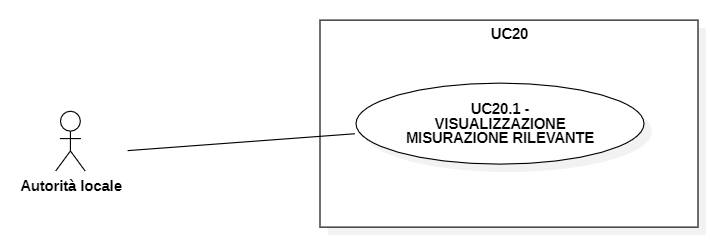
\includegraphics[width=0.9\textwidth]{../Images/subUC20.png}
    \caption{UC20.1 - VISUALIZZAZIONE MISURAZIONE RILEVANTE }
\end{figure}

%---------------------------- UC20.1 ---------------------------------

\subsubsection{UC20.1 - VISUALIZZAZIONE MISURAZIONE RILEVANTE}
\begin{itemize}
    \item \textbf{Attore principale:} Autorità locale;
    \item \textbf{Precondizioni:}
        \begin{itemize}
                \item L'autorità locale accede alla lista delle misurazioni rilevanti (UC20);
        \end{itemize}
    \item \textbf{Postcondizioni:}
        \begin{itemize}
                \item L'autorità locale visualizza una misurazione all'interno della lista delle misurazioni rilevanti.
        \end{itemize}
    \item \textbf{Scenario principale:}
        \begin{enumerate}
                \item Il sistema carica la lista delle misurazioni rilevanti.
        \end{enumerate}
\end{itemize}

%---------------------------- SUB_UC20.1 ---------------------------------

\begin{figure}[H]
    \centering
    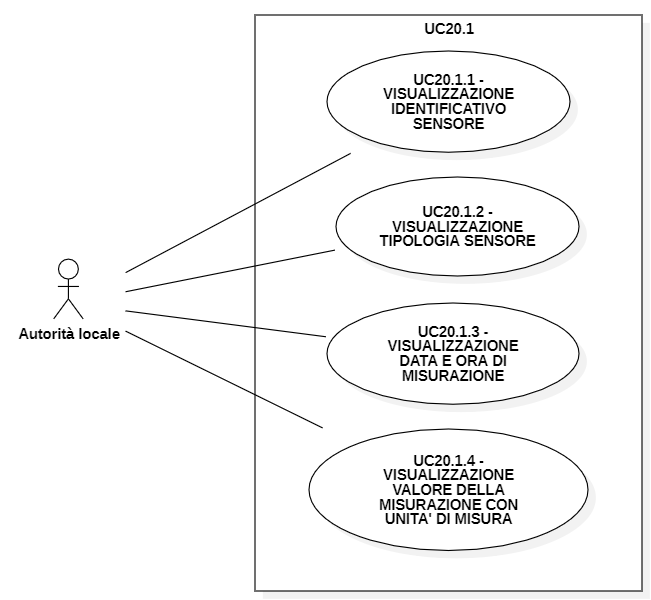
\includegraphics[width=0.9\textwidth]{../Images/subUC20.1.png}
    \caption{SOTTOCASI UC20.1 - VISUALIZZAZIONE MISURAZIONE RILEVANTE }
\end{figure}

%---------------------------- UC20.1.1 ---------------------------------

\subsubsection{UC20.1.1 - VISUALIZZAZIONE WIDGET LISTA RILEVANTI}
\begin{itemize}
      \item \textbf{Attore principale:} Autorità locale;
      \item \textbf{Precondizioni:}
            \begin{itemize}
                  \item Il sistema ha caricato la visualizzazione della dashboard (UC1);
            \end{itemize}
      \item \textbf{Postcondizioni:}
            \begin{itemize}
                  \item L'autorità locale visualizza la lista delle misurazioni rilevanti.
            \end{itemize}
      \item \textbf{Scenario principale:}
            \begin{enumerate}
                  \item L'autorità locale seleziona la visualizzione della lista delle misurazioni rilevanti.
            \end{enumerate}
      \item \textbf{User story associata:} \\
      Come autorità locale, desidero poter visualizzare una lista delle misurazioni rilevanti, al fine di reperire rapidamente delle misurazioni ritenute importanti.
\end{itemize}

%---------------------------- UC20.1.2 ---------------------------------

\subsubsection{UC20.1.2 - VISUALIZZAZIONE TIPOLOGIA SENSORE}
\begin{itemize}
    \item \textbf{Attore principale:} Autorità locale;
    \item \textbf{Precondizioni:}
        \begin{itemize}
                \item L'autorità locale visualizza una misurazione all'interno della lista delle misurazioni rilevanti (UC20.1);
        \end{itemize}
    \item \textbf{Postcondizioni:}
        \begin{itemize}
            \item L'autorità locale visualizza la tipologia del \textit{sensore}\textsubscript{\textit{G}} associato alla misurazione attualmente visualizzata all'interno della lista delle misurazioni rilevanti.
        \end{itemize}
    \item \textbf{Scenario principale:}
        \begin{enumerate}
            \item Il \textit{sistema}\textsubscript{\textit{G}} effettua il caricamento delle informazioni associate alla misurazione rilevante.
        \end{enumerate}
    \item \textbf{User story associata:} \\
    Come autorità locale, desidero poter visualizzare la tipologia del \textit{sensore}\textsubscript{\textit{G}} associato alla misurazione rilevante così da poter distinguere la tipologia della misurazione all'interno della lista delle misurazioni rilevanti, la quale contiene misurazioni provenienti da sensori di diversa tipologia.
\end{itemize}

%---------------------------- UC20.1.3 ---------------------------------

\subsubsection{UC20.1.3 - VISUALIZZAZIONE VALORE DELLA MISURAZIONE CON UNITÀ DI MISURA}
\begin{itemize}
    \item \textbf{Attore principale:} Autorità locale;
    \item \textbf{Precondizioni:}
        \begin{itemize}
                \item L'autorità locale visualizza una misurazione all'interno della lista delle misurazioni rilevanti (UC20.1);
        \end{itemize}
    \item \textbf{Postcondizioni:}
        \begin{itemize}
            \item L'autorità locale visualizza il valore con unità di misura della misurazione attualmente visualizzata all'interno della lista delle misurazioni rilevanti.
        \end{itemize}
    \item \textbf{Scenario principale:}
        \begin{enumerate}
            \item Il sistema effettua il caricamento delle informazioni associate alla misurazione rilevante.
        \end{enumerate}
    \item \textbf{User story associata:} \\
    Come autorità locale, desidero poter visualizzare il valore con unità di misura della misurazione rilevante.
\end{itemize}

%---------------------------- UC20.1.4 ---------------------------------

\subsubsection{UC20.1.4 - VISUALIZZAZIONE VALORE DELLA MISURAZIONE CON UNITÀ DI MISURA}
\begin{itemize}
    \item \textbf{Attore principale:} Autorità locale;
    \item \textbf{Precondizioni:}
        \begin{itemize}
                \item L'autorità locale visualizza una misurazione all'interno della lista delle misurazioni rilevanti (UC20.1);
        \end{itemize}
    \item \textbf{Postcondizioni:}
        \begin{itemize}
            \item L'autorità locale visualizza il valore con unità di misura della misurazione attualmente visualizzata all'interno della lista delle misurazioni rilevanti.
        \end{itemize}
    \item \textbf{Scenario principale:}
        \begin{enumerate}
            \item Il sistema effettua il caricamento delle informazioni associate alla misurazione rilevante.
        \end{enumerate}
    \item \textbf{User story associata:} \\
    Come autorità locale, desidero poter visualizzare il valore con unità di misura della misurazione rilevante.
\end{itemize}

%---------------------------- UC21 ---------------------------------
\newpage

\begin{figure}[H]
    \centering
    \includegraphics[width=0.9\textwidth]{../Images/uc21.PNG}
    \caption{UC21 - RIMOZIONE MISURAZIONE DA LISTA RILEVANTI }
\end{figure}
\subsubsection{UC21 - RIMOZIONE MISURAZIONE DA LISTA RILEVANTI}
\begin{itemize}
    \item \textbf{Attore principale:} Autorità locale;
    %\item \textbf{Descrizione:} L’autorità locale, dalla pagina adibita alla visione dei dati salvati tra i preferiti, rimuove un dato dalla lista.
    \item \textbf{Scenario principale:}
          \begin{enumerate}
            %  \item L'utente accede alla piattaforma per la visualizzazione della dashboard sullo stato della città o di una cella(UC1) (UC1.1);
             % \item L'utente sceglie di visualizzare la pagina dedicata alla visualizzazione dei dati preferiti;
              \item L'utente rimuove uno dei dati dalla lista.
          \end{enumerate}
    \item \textbf{Precondizioni:}
          \begin{itemize}
              \item  L'utente di trova nella pagina per la visulizzazione dei dati preferiti. (UC9)
              \item Almeno una misurazione è presente nella lista rilevanti.
          \end{itemize}
    \item \textbf{Postcondizioni:}
          \begin{itemize}
              \item  La misurazione viene rimosso dalla lista dei preferiti.
          \end{itemize}
    \item \textbf{User story associata:}
          \begin{itemize}
              \item Come autorità locale,
                    Desidero poter rimuovere un dato dalla lista dei preferiti sulla piattaforma,
                    Per poter gestire in modo efficiente i dati visualizzati sulla dashboard.
          \end{itemize}
\end{itemize}

%---------------------------- UC22 ---------------------------------

\begin{figure}[H]
    \centering
    \includegraphics[width=0.9\textwidth]{../Images/uc22.PNG}
    \caption{UC22 - VISUALIZZAZIONE ALLERTE SUPERAMENTO SOGLIE }
\end{figure}
\subsubsection{UC22 - VISUALIZZAZIONE ALLERTE SUPERAMENTO SOGLIE}
\begin{itemize}
      \item \textbf{Attore principale:} Autorità locale;
      \item \textbf{Precondizioni:}
            \begin{itemize}
                  \item Il sensore ha registrato una misurazione al di sopra o al di sotto di una soglia specifica.
            \end{itemize}
      \item \textbf{Postcondizioni:}
            \begin{itemize}
                  \item  L'autorità locale riceve una notifica di superamento di una soglia impostata.
            \end{itemize}
      \item \textbf{Scenario principale:}
            \begin{enumerate}
                  \item  Il sistema rileva condizioni che richiedono l'invio di una notifica per segnalare il superamento di una soglia impostata;
                  \item Il sistema inivia una notifica all'autorità locale.
            \end{enumerate}
      \item \textbf{User story associata:}
      Come autorità locale, desidero ricevere notifiche immediate nel caso in cui le misurazioni superino le soglie di sicurezza superiori o scendano al di sotto delle soglie di sicurezza inferiori, permettendomi di adottare prontamente azioni correttive e necessarie.
\end{itemize}

%---------------------------- UC23 ---------------------------------

\begin{figure}[H]
    \centering
    \includegraphics[width=0.9\textwidth]{../Images/uc23.PNG}
    \caption{UC23 - TRASMISSIONE DATI TEMPERATURA }
\end{figure}
\subsubsection{UC23 - TRASMISSIONE DATI TEMPERATURA}
\begin{itemize}
    \item \textbf{Attore principale:} Sensore;
    \item \textbf{Precondizioni:}
        \begin{itemize}
            \item Il \textit{sensore}\textsubscript{\textit{G}} è attivo e connesso al \textit{sistema}\textsubscript{\textit{G}}. 
        \end{itemize}
    \item \textbf{Postcondizioni:}
        \begin{itemize}
            \item Il \textit{sistema}\textsubscript{\textit{G}} ha memorizzato ed elaborato i dati inviati dal \textit{sensore}\textsubscript{\textit{G}}.
        \end{itemize}
    \item \textbf{Scenario principale:}
        \begin{enumerate}
            \item Il \textit{sensore}\textsubscript{\textit{G}} effettua un rilevamento della temperatura;
            \item Il \textit{sensore}\textsubscript{\textit{G}} formatta il messaggio da trasmettere al \textit{sistema}\textsubscript{\textit{G}} contenente l'identificativo del \textit{sensore}\textsubscript{\textit{G}} e la misurazione effettuata in gradi Celsius;
            \item Il \textit{sensore}\textsubscript{\textit{G}} trasmette il messaggio al \textit{sistema}\textsubscript{\textit{G}}.
        \end{enumerate}
    \item \textbf{User story associata:} \\
    Come Sensore, desidero trasmettere i rilevamenti di temperatura al \textit{sistema}\textsubscript{\textit{G}}.
\end{itemize}


%---------------------------- UC24 ---------------------------------

\begin{figure}[H]
    \centering
    \includegraphics[width=0.9\textwidth]{../Images/uc24.PNG}
    \caption{UC24 - TRASMISSIONE DATI UMIDITA' }
\end{figure}
\subsubsection{UC24 - TRASMISSIONE DATI UMIDITA'}
\begin{itemize}
    \item \textbf{Attore principale:} Sensore;
    \item \textbf{Precondizioni:}
        \begin{itemize}
            \item Il sensore è attivo e connesso al sistema. 
        \end{itemize}
    \item \textbf{Postcondizioni:}
        \begin{itemize}
            \item Il sistema ha memorizzato ed elaborato i dati inviati dal sensore.
        \end{itemize}
    \item \textbf{Scenario principale:}
        \begin{enumerate}
            \item Il sensore effettua un rilevamento dell'umidità nell'aria;
            \item Il sensore formatta il messaggio da trasmettere al sistema contenente l'identificativo del sensore e la misurazione effettuata in percentuale di umidità nell’aria;
            \item Il sensore trasmette il messaggio al sistema.
        \end{enumerate}
    \item \textbf{User story associata:} \\
    Come Sensore, desidero trasmettere i rilevamenti dell'umidità nell'aria al sistema.
\end{itemize}


%---------------------------- UC25 ---------------------------------

\begin{figure}[H]
    \centering
    \includegraphics[width=0.9\textwidth]{../Images/uc25.PNG}
    \caption{UC25 - TRASMISSIONE LIVELLO ACQUA }
\end{figure}
\subsubsection{UC25 - TRASMISSIONE DATI LIVELLO ACQUA}
\begin{itemize}
    \item \textbf{Attore principale:}Sensore;
    %\item \textbf{Descrizione:} L’autorità locale, dalla pagina adibita alla visione dei dati salvati tra i preferiti, rimuove un dato dalla lista.
    \item \textbf{Scenario principale:}
          \begin{enumerate}
              \item Il sensore effettua una rilevazione del livello dell'acqua;
              \item Il sensore formatta il messaggio da inviare al sistema;
              \item Il sensore invia il messaggio al sistema
          \end{enumerate}
    \item \textbf{Precondizioni:}
          \begin{itemize}
              \item  il sensore è attivito e connesso al sistema. 
          \end{itemize}
    \item \textbf{Postcondizioni:}
          \begin{itemize}
              \item  il sistema ha memorizzato ed elaborato i dati inviati dal sensore.
          \end{itemize}
    \item \textbf{User story associata:}
          \begin{itemize}
            \item  Come Sensore, voglio trasmettere in modo affidabile i dati di del livello dell'acqua al sistema, in modo che possano essere memorizzati e elaborati 
          \end{itemize}
\end{itemize}


%---------------------------- UC26 ---------------------------------

\begin{figure}[H]
    \centering
    \includegraphics[width=0.9\textwidth]{../Images/uc26.PNG}
    \caption{UC26 - TRASMISSIONE DATI ISOLE ECOLOGICHE }
\end{figure}
\subsubsection{UC26 - TRASMISSIONE DATI ISOLE ECOLOGICHE}
\begin{itemize}
    \item \textbf{Attore principale:}Sensore;
    %\item \textbf{Descrizione:} L’autorità locale, dalla pagina adibita alla visione dei dati salvati tra i preferiti, rimuove un dato dalla lista.
    \item \textbf{Scenario principale:}
          \begin{enumerate}
              \item Il sensore effettua una rilevazione sullo stato di riempimento delle isole ecologiche;
              \item Il sensore formatta il messaggio da inviare al sistema;
              \item Il sensore invia il messaggio al sistema
          \end{enumerate}
    \item \textbf{Precondizioni:}
          \begin{itemize}
              \item  il sensore è attivito e connesso al sistema. 
          \end{itemize}
    \item \textbf{Postcondizioni:}
          \begin{itemize}
              \item  il sistema ha memorizzato ed elaborato i dati inviati dal sensore.
          \end{itemize}
    \item \textbf{User story associata:}
          \begin{itemize}
            \item Come Sensore, voglio trasmettere in modo affidabile i dati di riempimento delle isole ecologiche al sistema, in modo che possano essere memorizzati e elaborati 
          \end{itemize}
\end{itemize}


%---------------------------- UC27 ---------------------------------

\begin{figure}[H]
    \centering
    \includegraphics[width=0.9\textwidth]{../Images/uc27.PNG}
    \caption{UC27 - TRASMISSIONE DATI COLONNINE DI RICARICA }
\end{figure}
\subsubsection{UC27 - TRASMISSIONE DATI COLONNINE DI RICARICA}
\begin{itemize}
    \item \textbf{Attore principale:} Sensore;
    \item \textbf{Precondizioni:}
        \begin{itemize}
            \item Il sensore è attivo e connesso al sistema. 
        \end{itemize}
    \item \textbf{Postcondizioni:}
        \begin{itemize}
            \item Il sistema ha memorizzato ed elaborato i dati inviati dal sensore.
        \end{itemize}
    \item \textbf{Scenario principale:}
        \begin{enumerate}
            \item Il sensore effettua un rilevamento sull'occupazione delle colonnine di ricarica;
            \item Il sensore formatta il messaggio da trasmettere al sistema;
            \item Il sensore trasmette il messaggio al sistema.
        \end{enumerate}
    \item \textbf{User story associata:} \\
    Come Sensore, desidero trasmettere con affidabilità i rilevamenti sull'occupazione delle colonnine di ricarica, garantendo che siano memorizzati e processati correttamente.
\end{itemize}

%---------------------------- UC28 ---------------------------------

\begin{figure}[H]
    \centering
    \includegraphics[width=0.9\textwidth]{../Images/uc28.PNG}
    \caption{UC28 - TRASMISSIONE DATI POLVERI SOTTILI }
\end{figure}
\subsubsection{UC28 - TRASMISSIONE DATI POLVERI SOTTILI}
\begin{itemize}
    \item \textbf{Attore principale:} Sensore;
    \item \textbf{Precondizioni:}
        \begin{itemize}
            \item Il sensore è attivo e connesso al sistema. 
        \end{itemize}
    \item \textbf{Postcondizioni:}
        \begin{itemize}
            \item Il sistema ha memorizzato ed elaborato i dati inviati dal sensore.
        \end{itemize}
    \item \textbf{Scenario principale:}
        \begin{enumerate}
            \item Il sensore effettua un rilevamento della quantità di particelle di polveri nell'aria;
            \item Il sensore formatta il messaggio da trasmettere al sistema;
            \item Il sensore trasmette il messaggio al sistema.
        \end{enumerate}
    \item \textbf{User story associata:} \\
    Come Sensore, desidero trasmettere i rilevamenti della quantità di particelle di polveri nell'aria al sistema.
\end{itemize}


%---------------------------- UC29 ---------------------------------

\begin{figure}[H]
    \centering
    \includegraphics[width=0.9\textwidth]{../Images/uc29.PNG}
    \caption{UC29 - TRASMISSIONE DATI GUASTI ELETTRICI }
\end{figure}
\subsubsection{UC29 - TRASMISSIONE DATI GUASTI ELETTRICI}
\begin{itemize}
    \item \textbf{Attore principale:} Sensore;
    \item \textbf{Precondizioni:}
        \begin{itemize}
            \item Il sensore è attivo e connesso al sistema. 
        \end{itemize}
    \item \textbf{Postcondizioni:}
        \begin{itemize}
            \item Il sistema ha memorizzato ed elaborato i dati inviati dal sensore.
        \end{itemize}
    \item \textbf{Scenario principale:}
        \begin{enumerate}
            \item Il sensore effettua un rilevamento della presenza di guasti elettrici;
            \item Il sensore formatta il messaggio da trasmettere al sistema;
            \item Il sensore trasmette il messaggio al sistema.
        \end{enumerate}
    \item \textbf{User story associata:} \\
    Come Sensore, desidero trasmettere i rilevamenti della presenza di guasti elettrici.
\end{itemize}


\newcounter{rowcounter}
\setcounter{rowcounter}{1}
